\chapter{Underwater granular flows}

\ifpdf
    \graphicspath{{Chapter6/figs/raster/}{Chapter6/figs/pdf/}{Chapter6/figs/}}
\else
    \graphicspath{{Chapter6/figs/vector/}{Chapter6/figs/}}
\fi

\section{Introduction}

Avalanches, landslides, and debris flows are geophysical hazards, which involve 
rapid mass movement of granular solids, water, and air as a single phase 
system. Globally, landslides 
cause billions of pounds in damage, and thousands of deaths and injuries each 
year. Hence, it is important to understand the triggering mechanism and the flow
evolution. The momentum transfer between the discrete and continuous 
phases significantly affects the dynamics of the flow as a 
whole~\citep{Topin2012}. Although certain macroscopic models are able to 
capture simple mechanical 
behaviours~\citep{Peker2007}, the complex physical mechanisms occurring at the 
grain scale, such as hydrodynamic instabilities, formation of clusters, 
collapse, and transport,~\citep{Topin2011} have largely been ignored. In 
particular, when the solid phase reaches a high volume fraction, the strong 
heterogeneity arising from the contact forces between the grains, and the 
hydrodynamic forces, are difficult to integrate into the homogenization process 
involving global averages. 

In order to describe the mechanism of immersed 
granular flows, it is important to consider both the dynamics of the solid 
phase and the role of the ambient fluid~\citep{Denlinger2001}. The dynamics of 
the solid phase alone is insufficient to describe the mechanism of granular 
flow in a fluid. It is important to consider the effect of hydrodynamic forces 
that reduce the weight of the solids inducing a transition from dense-compacted 
to dense-suspended flows, and the drag interactions which counteract the 
movement of the solids~\citep{Meruane2010}. Transient regimes characterized by 
change in the solid fraction, dilation at the onset of flow and development of 
excess pore pressure, result in altering the balance between the stress carried 
by the fluid and that carried by the grains, thereby changing the overall 
behaviour of the flow. 


The presence of a fluid phase in a granular medium has profound effects on its 
mechanical behaviour. In dry granular media the rheology is governed by grain 
inertia and static stresses sustained by the contact network depending on the 
shear-rate and confining pressure, respectively~\citep{Midi2004}. As the fluid 
inertia and viscosity come into play, complications arise as a result of 
contradictory effects. On one hand, the fluid may delay the onset of
granular flow or prevent the dispersion of the grains by
developing negative pore pressures~\citep{Pailha2008,Topin2011}. On the other
hand, the fluid lubricates the contacts between grains, enhancing in this way 
the granular flow, and it has a retarding effect at the same time by inducing 
drag forces on the grains. The objective of the present study is to understand 
the differences in the mechanism of flow initiation and kinematics between dry 
and submerged granular flow. In the present study, 2D Lattice-Boltzmann and 
Discrete Element Method is used to model the fluid-soil interactions in  
underwater granular flows.

\section{Granular collapse in fluid}

The collapse of a granular column, which mimics the
collapse of a cliff, has been extensively studied in the case of
dry granular material, when the interstitial fluid plays no
role (see~\cref{sec:dry_granular_column}). The problem of the granular collapse 
in a liquid,which is of importance for submarine landslides, has to our
knowledge attracted less attention~\citep{Rondon2011}.~\citet{THOMPSON2007} 
observed that the presence of liquid dramatically changes the way a granular 
column collapses compared to the dry case. The destabilization of a granular 
pile strongly depends on the initial volume fraction of the packing. For dense 
packings the granular flow is localized at the free surface of the pile, 
whereas for loose packings the destabilization occurs in the bulk of the
material and has a parabolic profile~\citep{Bonnet2010,Topin2011,Iverson2000}. 
In the present study, the collapse of a granular column in fluid is studied 
using 2D LBM - DEM and the flow kinematics is compared with dry granular 
collapse. The role of permeability and initial volume fraction on the run-out 
behaviour is also investigated.  

\subsection{LBM-DEM Coupling}

Lattice Boltzmann approach can accommodate large grain sizes and the 
interaction between the fluid and the moving grains can be modelled through 
a relatively simple fluid – grain interface treatment. Further, employing the 
Discrete Element Method (DEM) to account for the grain – grain interaction 
naturally leads to a combined LB – DEM procedure~\citep{Mansouri2009}. 

In this study, a 2D poly-disperse system ($d_{max}/d_{min} = 1.8$) of circular 
discs in fluid is used to simulate the behaviour of granular collapse in 
fluid (see~\Cref{fig:geometry}). A cumulative $\beta$ distribution is adopted 
to generate grains with $d_{max}$ and $d_{min}$ as 1.25~\si{\mm} and 
2.2~\si{\mm}, respectively. The soil column is modelled using 
$\approx 2000$ discs of density \SI{2650}{\kg\per\cubic\meter} and a contact 
friction angle of \SI{26}{\degree}. A linear-elastic contact model is used in 
DEM simulations. The collapse of the column was simulated inside a fluid with a 
density of \SI{1000}{\kg\per\cubic\meter}  and a kinematic viscosity of 
\SI{1e-6}{\square\meter\per\second}. The gravity angle $\theta$ is set to 
zero to simulate collapse onto a horizontal surface. The choice of a 2D 
geometry has the advantage of cheaper computational effort than a 3D case, 
making it feasible to simulate very large systems. 

\begin{figure}[htpb]
\centering
\includegraphics[width=0.97\columnwidth]{geometry}
\caption{Underwater granular collapse set-up.}
\label{fig:geometry}
\end{figure}

The Eulerian nature of the LBM formulation, together with the common explicit 
time step scheme of both LBM and DEM makes this coupling strategy an efficient 
numerical procedure for the simulation of grain – fluid systems. The critical 
time step for DEM is computed based on the local contact natural frequency and 
damping ratio. A sub-cycling time integration is adopted in DEM 
(see~\cref{sec:coupled_lbm_dem}). A fluid flow (LBM) time step, $\Delta t = 
2.0E^-5s$ is determined based on the viscosity and relaxation parameter $\tau = 
0.506$. An integer ratio $n_s$, between the fluid flow time step $\Delta t$ and 
DEM time step $\Delta t_D$ is determined as 15, i.e., every LBM iteration 
involves a sub-cycle of 15 DEM iterations.

In order to capture realistic physical behaviour of the fluid – grain system, 
it is essential to model the boundary condition between the fluid and the grain 
as a non-slip boundary condition, i.e. the fluid near the grain should have 
similar velocity as the grain boundary. The solid grains inside the fluid are 
represented by lattice nodes. The discrete nature of lattice, results in a 
stepwise representation of the surfaces (see~\cref{fig:LBM-DEM}), which are 
circular, hence sufficiently small lattice spacing $h$ is required. The 
smallest DEM grain in the system controls the length of the lattice spacing. In 
the present study, a very fine discretisation of $d_{min}/h = 10$ is adopted, 
i.e., the smallest grain with a  diameter $d_min$ in the system is discretised 
into 100 lattice nodes ($ 10h \times 10h$). This represents a very accurate 
representation of the interaction between the solid and the fluid nodes.

\begin{figure}[htpb]
\centering
\includegraphics[width=0.97\textwidth]{LBM-DEM}
\caption{Discretisation of solid grains in LBM grid. Shows the step-wise 
representation of circular disks in the lattice.}
\label{fig:LBM-DEM}
\end{figure}


\subsection{Permeability}

In DEM, the grain – grain interaction is described based on the contact 
interactions. In a 3D granular assembly, the pore spaces between grains are 
interconnected, whereas in a 2-D assembly, the grains are in contact with each 
other and this results in a non-interconnected pore-fluid space. Which means 
that the pore-fluid enclosed between the grains cannot flow to neighbouring 
pore-space.  This results in a unnatural no flow condition in a 2-D case 
(see~\cref{fig:reduction}). In 
order to overcome this difficulty, a 
reduction in radius is assumed only during LBM computations (fluid and fluid – 
solid interaction). The reduced radius of the soil grain, i.e., the 
\textit{hydrodynamic radius} `r', allows for interconnected pore space through 
which the pore-fluid can flow similar to 3D behaviour. The reduction in radius 
is assumed only during LBM computations, hence this technique has no effect on 
the grain – grain interactions computed using DEM. 

\begin{figure}[htpb]
\centering
\includegraphics[width=0.45\textwidth]{reduction}
\caption{Schematic representation of the hydrodynamic radius in LBM-DEM 
computation}
\label{fig:reduction}
\end{figure}

Realistically, the hydrodynamic radius can be varied from $ r = 0.7 R$ to 
$0.95R$, where ‘R’ is the grain radius. Different permeability can be 
obtained, for any given initial packing, by varying the hydrodynamic radius of 
the grains, without changing the actual granular packing. Hence, the 
hydrodynamic radius represents the permeability of the granular assembly. In 
another sense, the hydrodynamic radius can be assumed to represent the 
irregularities on the granular surface. Reducing the hydrodynamic radius 
represents wider channel and more flow between the grains. 

In order to understand the relation between the hydrodynamic radius and the 
permeability of the granular assembly, horizontal permeability tests are 
performed by varying the hydrodynamic radius as 0.7R, 0.75R, 0.8R, 0.85R, 0.9 
and 0.95R. A square sample of $50~\si{\mm} \times 50~\si{\mm}$ is used to 
determine the transverse permeability. Dirichlet boundary condition (discussed 
in~\cref{sec:lbm_bc}), i.e.,  pressure/density constrain is applied along the 
left and the right boundaries. The density on the left boundary is increased in 
small increments ($10^{-4} \Delta P$), which a constant density is maintained 
on the right boundary. This results in a pressure gradient causing the fluid to 
flow (see~\cref{fig:perm}). 

 
\begin{figure}[tbhp]
	\centering
	\begin{subfigure}[b]{0.475\textwidth}
		\centering
		\includegraphics[width=\textwidth]{Pressure}
		\caption{Pressure gradient in the granular assembly}
		\label{fig:pressure}
	\end{subfigure}
	\begin{subfigure}[b]{0.475\textwidth}
		\centering
		\includegraphics[width=0.8\textwidth]{Velocity}
		\caption{Horizontal flow due to pressure gradient}
		\label{fig:velocity}
	\end{subfigure}
	\caption{Evaluation of the horizontal permeability for a 
	hydrodynamic radius of 0.7R.}
	\label{fig:perm}
\end{figure}


The mean velocity of flow (v) 
is determined and the permeability of the sample (k) is computed as:
%
\begin{equation}
k=v\cdot\mu\cdot\frac{\Delta x}{\Delta P} \,,
\end{equation}
%
where $\mu$ is the dynamic viscosity of the fluid (\si{\Pa\s}), $\Delta x$ is 
the thickness of the bed of porous medium \si{\m}, and $\Delta P$ is the 
applied pressure difference \si{\Pa}. For a given hydrodynamic radius, the 
pressure gradient $\Delta P$ is varied to obtain different flow rates. Probing 
the fluid space showed a Poiseuille flow behaviour between grains. The flow is 
still within the Darcy's laminar flow regime, which is verified by the linear 
slope between the pressure gradient and mean flow velocity 
(see~\cref{fig:permeability}). It can be observed that with increase in the 
hydrodynamic radius the permeability decreases, i.e., the slope of the mean 
flow velocity 
to the pressure gradient decreases. At very low pressure gradient ($\Delta P 
\le 0.1$), both 0.9R and 0.95r has a no flow condition. A hydrodynamic radius 
of $r = 0.95R$ shows almost no flow behaviour, even at higher pressure 
gradients. A high value of hydrodynamic radius $r > 0.95R$ 
results in unnatural flow behaviour. Hence, hydrodynamic radii in the range of 
0.7 to 0.95R are adopted in the present study.

\begin{figure}[htpb]
\centering
\includegraphics[width=0.95\textwidth]{permeability}
\caption{Variation of the mean flow velocity with pressure gradient for 
different hydrodynamic radius.}
\label{fig:permeability}
\end{figure}


Increase in the hydrodynamic radius from 0.7 to 0.95 reduces the porosity from 
0.60 to 0.27. The permeability computed from LB – DEM method is verified by 
comparing it with the analytical solution. One of the widely used analytical 
solution for permeability is the Carman – Kozeny equation (CK Model), 
which is based on the Poiseuille flow through a pipe and is mainly used for 3D, 
homogeneous, isotropic, granular porous media at moderate porosities. In the 
present study, a modified Carman – Kozeny equation that takes into account the 
micro-structure of the fibres and that is valid in a wide range of porosities 
is adopted~\citep{Yazdchi2011}. The normalized permeability is defined as
\begin{equation}
\frac{k}{d^2} = \frac{\epsilon}{\psi_{CK}(1-\epsilon)^2} \,.
\end{equation}
%
In the CK model, the hydraulic diameter $D_h$ , is expressed as a function of 
measurable quantities: porosity and specific surface area
%
\begin{align}
D_h & = \frac{4\epsilon V}{S_v}=\frac{\epsilon d}{(1 - \epsilon)} \,, \\
a_v & = \frac{\mbox{grain surface}}{\mbox{grain volume}} = 
\frac{S_v}{(1-\epsilon V)} = \frac{4}{d} \,,
\end{align}
%
where $S_v$ is the total wetted surface, and $a_v$ is the specific surface 
area. The above value of $a_v$ is for circles (cylinders) - for spheres $a_v = 
6/d$. $\psi_{CK}$ is the empirically  measured CK factor, which represents both 
the shape factor and the deviation of flow direction from that in a duct. It is 
approximated for randomly packed beds of spherical grains. The normalized 
permeability for different porosity obtained by varying the radius from 0.7 to 
0.95 is presented in~\cref{fig:Carman}. The normalized permeability is found to 
match the qualitative trend of the Carman-Kozeny equations. The LB – DEM 
permeability curve lies between the permeability curves for spherical and 
cylindrical grain arrangements implying a better approximation of permeability 
in 2D granular assembly by reducing the radius during LBM computations.

\begin{figure}[htpb]
\centering
\includegraphics[width=0.95\textwidth]{Carman}
\caption{Relation between permeability and porosity for 
different hydrodynamic radius and comparison with the analytical solution.}
\label{fig:Carman}
\end{figure}

\subsection{Collapse in fluid: Flow evolution}
Two-dimensional plane-strain LBM-DEM simulations of granular column 
collapse are performed by varying the initial aspect ratio of the column from 
0.2 to 6. A hydrodynamic radius of 0.7R is adopted during LBM computations.  
The granular assemble has a packing fraction of $83\%$. The normalized final 
run-out distance is computed as $\Delta L = 
(L_{\textit{f}}-L_{\textit{0}})/L_{\textit{0}}$. Similar to dry granular 
collapse, the duration of collapse is normalised with a criticial time $\tau_c 
= \sqrt{H/g}$. Where, $H$ is the initial height of the granular column and g is 
the acceleration due to gravity.  Dry and buoyant analyses of granular column 
collapse are also performed to understand the effect of hydrodynamic forces on 
the run-out distance.

Snapshots of flow evolution of a granular column collapse with an initial 
aspect ratio of 0.4 is shown in~\cref{fig:a04_snapshots}. The failure begins at 
the toe end of the column, and the fracture surface propagates into the column 
at an angle of about $50\si{\degree}$, similar to dry column. For the short 
column, the failure is due to collapse of the flanks. Once the material is 
destabilisied, the granular mass interacts with the surrounding fluid resulting 
in formation of turbulent vortices. These vortices interact with the grains at 
the surface, resulting in irregularities on the free surface. Force chains can 
be observed in the static region of collapse, which indicates the flow can be 
described using a continuum theory. As the granular material ceases to flow, 
force chains develop at the flow front, revealing consolidation of the granular 
mass resulting in increase in strength. 

\begin{figure}
\makebox[\linewidth][c]{
\begin{subfigure}[b]{0.95\textwidth}
	\centering
    \includegraphics[width=0.95\textwidth]{a04/a04_0}
    \caption{$t = 0\tau_c$}
    \label{fig:a04_0}
\end{subfigure}
}\\

\makebox[\linewidth][c]{
\begin{subfigure}[b]{0.95\textwidth}
	\centering
    \includegraphics[width=0.95\textwidth]{a04/a04_tc}
    \caption{$t = 1\tau_c$}
    \label{fig:a04_tc}
\end{subfigure}
}\\

\makebox[\linewidth][c]{
\begin{subfigure}[b]{0.95\textwidth}
	\centering
    \includegraphics[width=0.95\textwidth]{a04/a04_3tc}
    \caption{$t = 3\tau_c$}
    \label{fig:a04_3tc}
\end{subfigure}
}\\

\makebox[\linewidth][c]{
\begin{subfigure}[b]{0.95\textwidth}
	\centering
    \includegraphics[width=0.95\textwidth]{a04/a04_6tc}
    \caption{$t = 6\tau_c$}
    \label{fig:a04_6tc}
\end{subfigure}
}\\

\makebox[\linewidth][c]{
\begin{subfigure}[b]{0.95\textwidth}
	\centering
    \includegraphics[width=0.95\textwidth]{a04/a04_8tc}
    \caption{$t = 8\tau_c$}
    \label{fig:a04_8tc}
\end{subfigure}
}
\caption{Flow evolution of a granular column collapse in fluid (a = 0.4). Shows 
the velocity profile of fluid due to interaction with the grains (red - higher 
velocity).}
\label{fig:a04_snapshots}
\end{figure}


The evolution of run-out with time for a short column (a = 0.4) is presented 
in~\cref{fig:Runout_a04f}. The dry column exhibits longer run-out distance in 
comparison to the submerged column. The collapse of a dry column using DEM 
represents a collapse in vacuum, without any influence of drag forces or 
viscosity of air. A LBM-DEM simulation of a granular column collapse using the 
kinematic viscosity of air is performed to compare the dry column with the 
collapse in air. It can be observed that both the ``dry'' condition and the 
collapse in air show almost the same run-out behaviour. However, the collapse 
in fluid (water) results in a much shorter run-out distance. The granular mass 
in fluid has the buoyant mass, in contrast to the dry density. A dry granular 
collapse with the buoyant unit weight is performed to understand the effect of 
buoyancy on the run-out behaviour. The dry column with buoyant unit weight also 
exhibits longer run-out behaviour than the collapse in fluid. However, due to 
decrease in the initial potential energy, the run-out observed in the buoyant 
condition is shorter than the dry condition. The column collapse in fluid takes 
longer to evolve when submerged in water, which might be due to the development 
of large negative porewater pressure that is generated during the shear failure 
along the fracture surface. The large negative pore pressure has to be 
dissipated before the granular mass above the fracture surface can collapse and 
flow. The shorter run-out distance in the fluid case, in comparison with the 
dry and buoyant conditions, shows that the collapse in fluid is significantly 
affected by the hydrodynamic drag force acting on the soil grains. The 
evolution of height $H/L$ is presented in~\cref{}. Since the failure of the 
column is only at the flank, the central static region remains unaffected. 
Hence, the final height of the column is the same in dry and submerged 
conditions.

\begin{figure}[htpb]
\centering
\includegraphics[width=0.9\textwidth]{Runout_a04f}
\caption{Evolution of run-out for a column collapse in fluid (a = 0.4)}
\label{fig:Runout_a04f}
\end{figure}

\begin{figure}[htpb]
\centering
\includegraphics[width=0.9\textwidth]{Height_a04f}
\caption{Evolution of height with time for a column collapse in fluid 
(a = 0.4)}
\label{fig:Height_a04f}
\end{figure}

The evolution of normalised kinetic energy with time for a column with an 
initial aspect ratio of 0.4 is shown in~\cref{fig:a04f_energy}. It can be 
observed that the peak kinetic energy is attained later in the submerged 
condition than the dry collapse. This can be attributed to the time required to 
overcome the negative pore pressure generated during the shear along the 
fracture surface. For short columns the critical time $\tau_c$ is controlled by 
the vertical kinetic energy. The amount of kinetic energy in submerged case is 
significanlty lower than the dry condition. Also, the potential energy 
evolution (see~\cref{fig:PE_a04f}) shows a significant influence of the 
hydrodynamic forces on the amount of material destabilised during the collapse. 
The drag forces reduces and slows down the amount of material that undergo 
collapse resulting in shorter run-out distance for short columns. 
\begin{figure}
\centering
\makebox[\linewidth][c]{
\begin{subfigure}[t]{0.8\textwidth}
	\centering
    \includegraphics[width=\textwidth]{KE_a04f}
    \caption{Evolution of the total kinetic energy}
    \label{fig:KE_a04f}
\end{subfigure}
}\\
\makebox[\linewidth][c]{
\begin{subfigure}[t]{0.95\textwidth}
	\centering
    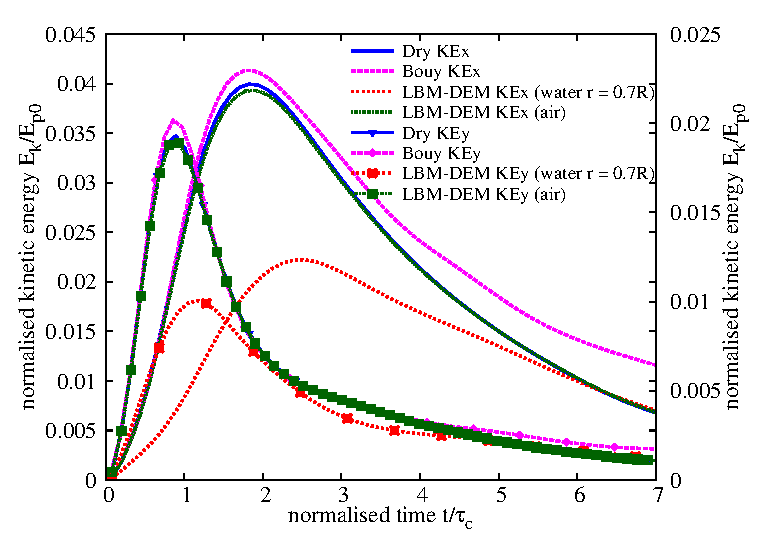
\includegraphics[width=\textwidth]{KExy_a04f}
    \caption{Evolution of horizontal and vertical kinetic energies}
    \label{fig:KExy_a04f}
\end{subfigure}
}
\caption{Evolution of kinetic energies with time for a granular column collapse 
in fluid (a = 0.4)}
\label{fig:a04f_energy}
\end{figure}

\begin{figure}
	\centering
    \includegraphics[width=0.9\textwidth]{PE_a04f}
    \caption{Evolution of the potential energy with time for a granular column 
    collapse in fluid (a = 0.4)}
    \label{fig:PE_a04f}
\end{figure}

Snapshots of flow evolution of a granular column collapse with an initial 
aspect ratio of 4 is shown in~\cref{fig:a4_snapshots}. 

\begin{figure}
\makebox[\linewidth][c]{
\begin{subfigure}[b]{0.95\textwidth}
	\centering
    \includegraphics[width=0.95\textwidth]{a4/a4_0}
    \caption*{$t = 0\tau_c$}
    \label{fig:a4_0}
\end{subfigure}
}\\

\makebox[\linewidth][c]{
\begin{subfigure}[b]{0.95\textwidth}
	\centering
    \includegraphics[width=0.95\textwidth]{a4/a4_tc}
    \caption*{$t = 1\tau_c$}
    \label{fig:a4_tc}
\end{subfigure}
}\\
\makebox[\linewidth][c]{
\begin{subfigure}[b]{0.95\textwidth}
	\centering
    \includegraphics[width=0.95\textwidth]{a4/a4_3tc}
    \caption*{$t = 3\tau_c$}
    \label{fig:a4_3tc}
\end{subfigure}
}
\end{figure}
\begin{figure}
\ContinuedFloat
\makebox[\linewidth][c]{
\begin{subfigure}[b]{0.95\textwidth}
	\centering
    \includegraphics[width=0.95\textwidth]{a4/a4_6tc}
    \caption*{$t = 6\tau_c$}
    \label{fig:a4_6tc}
\end{subfigure}
}\\
\makebox[\linewidth][c]{
\begin{subfigure}[b]{0.95\textwidth}
	\centering
    \includegraphics[width=0.95\textwidth]{a4/a4_8tc}
    \caption*{$t = 8\tau_c$}
    \label{fig:a4_8tc}
\end{subfigure}
}
\caption{Flow evolution of a granular column collapse in fluid (a = 4). Shows 
the velocity profile of fluid due to interaction with the grains (red - higher 
velocity).}
\label{fig:a4_snapshots}
\end{figure}


\begin{figure}[htpb]
\centering
\includegraphics[width=0.9\textwidth]{Runout_a4f}
\caption{Evolution of run-out for a column collapse in fluid (a = 4)}
\label{fig:Runout_a4f}
\end{figure}

\begin{figure}[htpb]
\centering
\includegraphics[width=0.9\textwidth]{Height_a4f}
\caption{Evolution of height with time for a column collapse in fluid 
(a = 4)}
\label{fig:Height_a4f}
\end{figure}

\begin{figure}
\centering
\makebox[\linewidth][c]{
\begin{subfigure}[t]{0.8\textwidth}
	\centering
    \includegraphics[width=\textwidth]{KE_a4f}
    \caption{Evolution of the total kinetic energy}
    \label{fig:KE_a4f}
\end{subfigure}
}\\
\makebox[\linewidth][c]{
\begin{subfigure}[t]{0.95\textwidth}
	\centering
    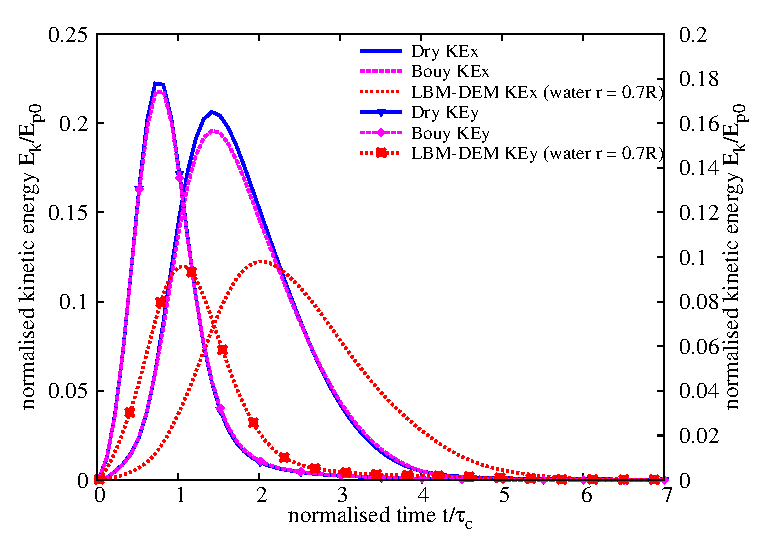
\includegraphics[width=\textwidth]{KExy_a4f}
    \caption{Evolution of horizontal and vertical kinetic energies}
    \label{fig:KExy_a4f}
\end{subfigure}
}
\caption{Evolution of kinetic energies with time for a granular column collapse 
in fluid (a = 4)}
\label{fig:a4f_energy}
\end{figure}

\begin{figure}
	\centering
    \includegraphics[width=0.9\textwidth]{PE_a4f}
    \caption{Evolution of the potential energy with time for a granular column 
    collapse in fluid (a = 4)}
    \label{fig:PE_a4f}
\end{figure}

\begin{figure}[tbhp]
	\centering
	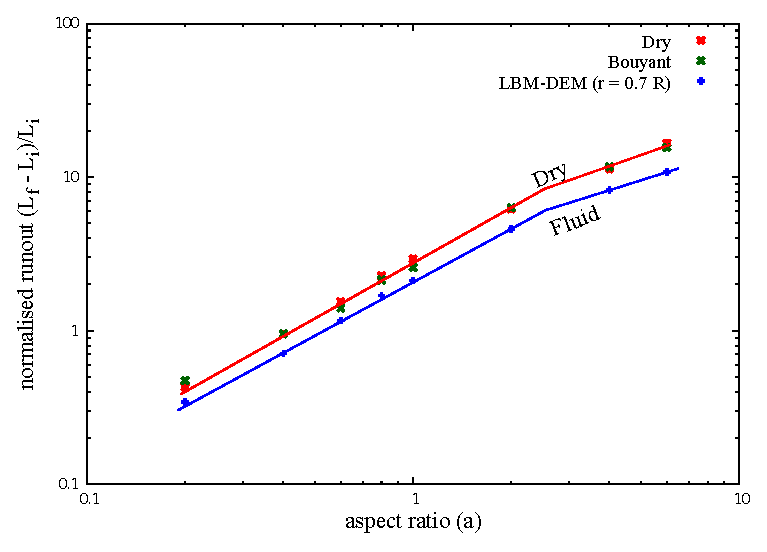
\includegraphics[width=\textwidth]{runoutf}
	\caption{Normalised final run-out distance for columns with different 
	initial aspect ratios. Comparison of dry and submerged granular column 
	collapse.}
	\label{fig:runoutf}
\end{figure}

\begin{figure}[tbhp]
	\centering
	\includegraphics[width=0.975\textwidth]{Heightf}
	\caption{Normalised final collapse height for columns with different 
	initial aspect ratios. Comparison of dry and submerged granular column 
	collapse.}
	\label{fig:heightf}
\end{figure}

\subsection{Effect of permeability}

\begin{figure}
\makebox[\linewidth][c]{
\begin{subfigure}[b]{0.95\textwidth}
	\centering
    \includegraphics[width=0.95\textwidth]{a08/a08r07_dense}
    \caption{High permeability (r = 0.7 R)}
    \label{fig:a08r07_dense}
\end{subfigure}
}\\
\makebox[\linewidth][c]{
\begin{subfigure}[b]{0.95\textwidth}
	\centering
    \includegraphics[width=0.95\textwidth]{a08/a08r095_dense}
    \caption{Low permeability (r = 0.95 R)}
    \label{fig:a08r095_dense}
\end{subfigure}
}
\caption{Effect of permeability on the deposit morphology of a granular column 
collapse in fluid (a = 0.8)}
\label{fig:a08_dense_snapshots}
\end{figure}


\begin{figure}[htpb]
\centering
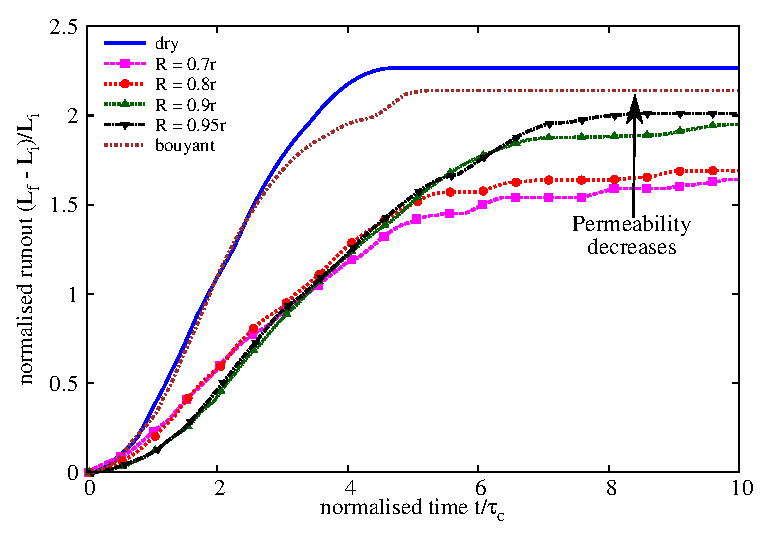
\includegraphics[width=0.9\textwidth]{Runout_a08_dense}
\caption{Effect of permeability on the evolution of run-out for a column 
collapse in fluid (a = 0.8)}
\label{fig:Runout_a08_dense}
\end{figure}

\begin{figure}
\centering
\makebox[\linewidth][c]{
\begin{subfigure}[t]{0.8\textwidth}
	\centering
    \includegraphics[width=\textwidth]{KE_a08_dense}
    \caption{Evolution of the total kinetic energy}
    \label{fig:KE_a08_dense}
\end{subfigure}
}\\
\makebox[\linewidth][c]{
\begin{subfigure}[t]{0.95\textwidth}
	\centering
    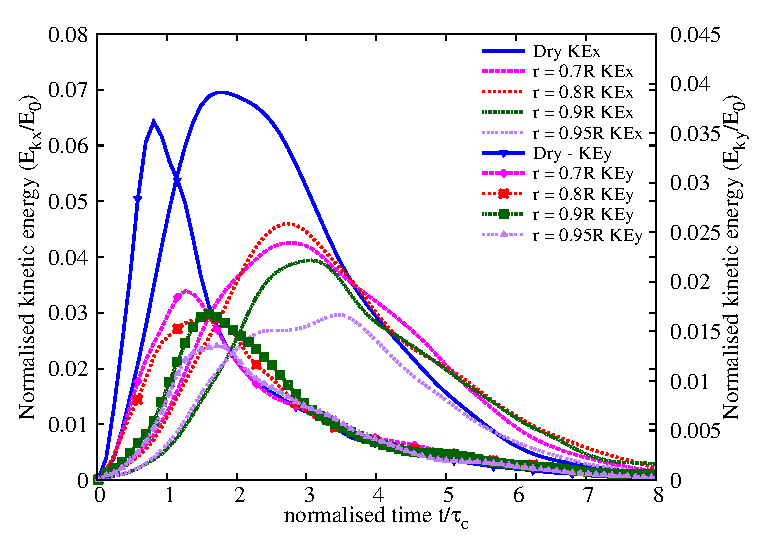
\includegraphics[width=\textwidth]{KExy_a08_dense}
    \caption{Evolution of horizontal and vertical kinetic energies}
    \label{fig:KExy_a08_dense}
\end{subfigure}
}
\caption{Effect of permeability on the evolution of kinetic energies with time 
for a granular column collapse in fluid (a = 0.8)}
\label{fig:a08_dense_energy}
\end{figure}

\begin{figure}
	\centering
    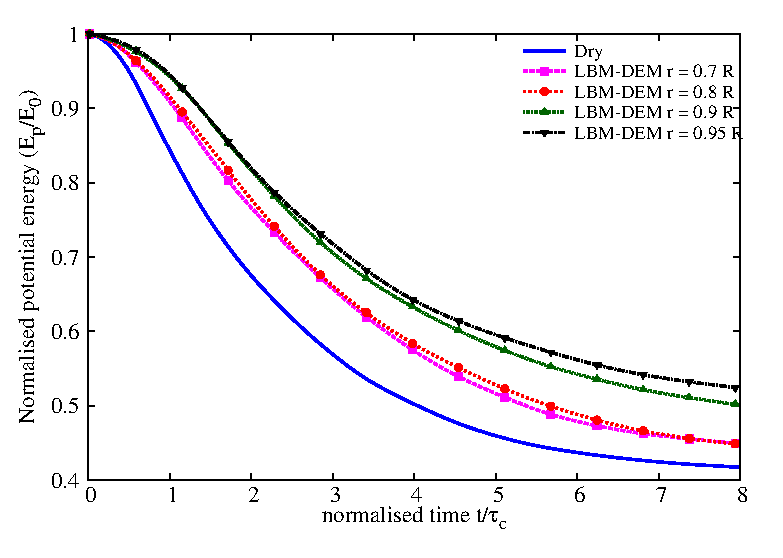
\includegraphics[width=0.9\textwidth]{PE_a08_dense}
    \caption{Effect of permeability on the evolution of the potential energy 
    with time for a granular column collapse in fluid (a = 0.8)}
    \label{fig:PE_a08_dense}
\end{figure}

\begin{figure}
	\centering
    \includegraphics[width=0.9\textwidth]{Packing_Density_a08_dense}
    \caption{Effect of permeability on the evolution of packing density for a 
    granular column collapse in fluid (a = 0.8 \& dense initial packing)}
    \label{fig:Packing_Density_a08_dense}
\end{figure}

\begin{figure}[tbhp]
	\centering
	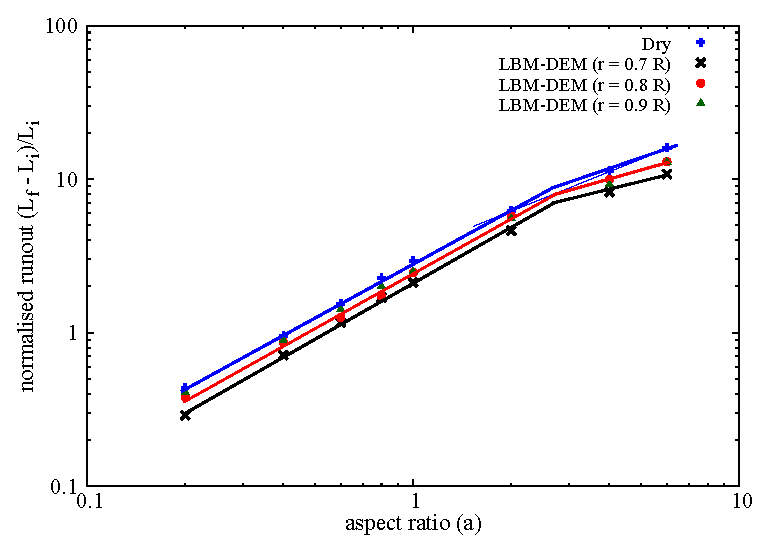
\includegraphics[width=\textwidth]{runout_fluid_dry}
	\caption{Normalised final run-out distance for columns with different 
	initial aspect ratios. Comparison of dry and submerged granular column 
	collapse for different hydrodynamic radius (0.7R, 0.8R and 0.9R).}
	\label{fig:runout_fluid_dry}
\end{figure}

\begin{figure}[tbhp]
	\centering
	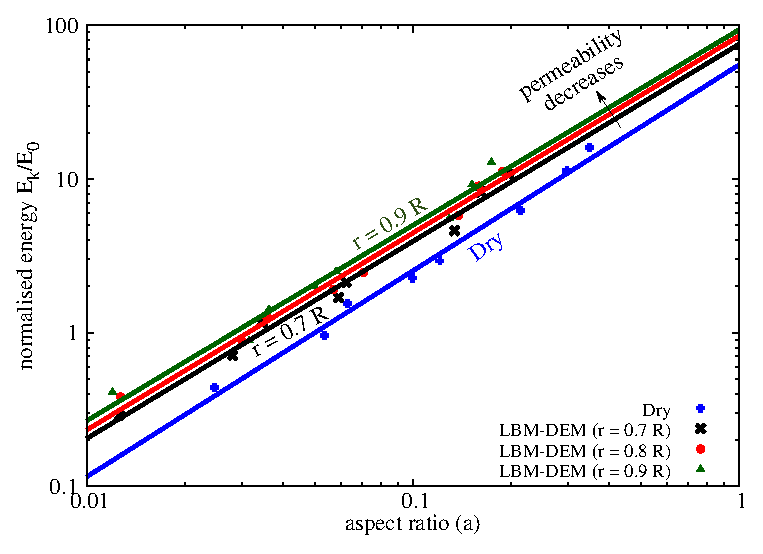
\includegraphics[width=\textwidth]{runout_fluid_dry_energy}
	\caption{Normalised final run-out distance for columns as a function of 
	peak kinetic energy. Comparison of dry and submerged granular column 
	collapse for different hydrodynamic radius (0.7R, 0.8R and 0.9R).}
	\label{fig:runout_fluid_dry_energy}
\end{figure}

\clearpage
\subsection{Effect of initial packing density}

\begin{figure}
\centering
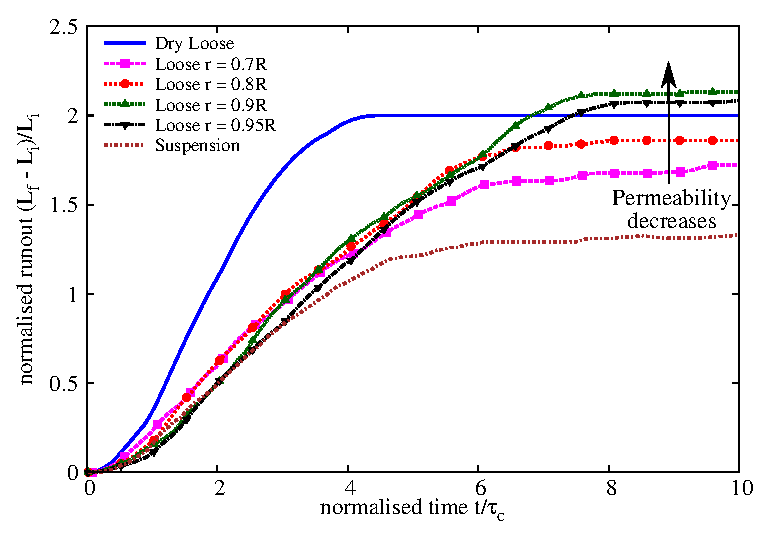
\includegraphics[width=0.9\textwidth]{Runout_a08_loose}
\caption{Effect of permeability on the evolution of run-out for a column 
collapse in fluid (a = 0.8 \& loose packing)}
\label{fig:Runout_a08_loose}
\end{figure}

\begin{figure}
\centering
\makebox[\linewidth][c]{
\begin{subfigure}[t]{0.975\textwidth}
	\centering
    \includegraphics[width=\textwidth]{a08/Loose_r07_PWP_ini}
    \caption{High permeability (r = 0.7 R)}
    \label{fig:Loose_r07_PWP_ini}
\end{subfigure}
}\\
\makebox[\linewidth][c]{
\begin{subfigure}[t]{0.975\textwidth}
	\centering
    \includegraphics[width=\textwidth]{a08/Loose_r095_PWP_ini}
    \caption{Low permeability (r = 0.95 R)}
    \label{fig:Loose_r095_PWP_ini}
\end{subfigure}
}
\caption{Effect of permeability on the excess pore water pressure distribution 
for a granular column collapse in fluid (a = 0.8 \& loose packing) at $t = 
\tau_c$}
\label{fig:Loose_PWP_ini}
\end{figure}

\begin{figure}
\centering
\makebox[\linewidth][c]{
\begin{subfigure}[t]{0.975\textwidth}
	\centering
    \includegraphics[width=\textwidth]{a08/Loose_r07_PWP_flow}
    \caption{High permeability (r = 0.7 R)}
    \label{fig:Loose_r07_PWP_flow}
\end{subfigure}
}\\
\makebox[\linewidth][c]{
\begin{subfigure}[t]{0.975\textwidth}
	\centering
    \includegraphics[width=\textwidth]{a08/Loose_r095_PWP_flow}
    \caption{Low permeability (r = 0.95 R)}
    \label{fig:Loose_r095_PWP_flow}
\end{subfigure}
}
\caption{Effect of permeability on the excess pore water pressure distribution 
for a granular column collapse in fluid (a = 0.8 \& loose packing) at $t = 
2\tau_c$}
\label{fig:Loose_PWP_flow}
\end{figure}


\begin{figure}
\centering
\makebox[\linewidth][c]{
\begin{subfigure}[t]{0.975\textwidth}
	\centering
    \includegraphics[width=\textwidth]{a08/LBM_MD_loose_a08_r07_pt}
    \caption{High permeability (r = 0.7 R)}
    \label{fig:LBM_MD_loose_a08_r07_pt}
\end{subfigure}
}\\
\makebox[\linewidth][c]{
\begin{subfigure}[t]{0.975\textwidth}
	\centering
    \includegraphics[width=\textwidth]{a08/LBM_MD_a08_Loose_r09}
    \caption{Low permeability (r = 0.95 R)}
    \label{fig:LBM_MD_a08_Loose_r09}
\end{subfigure}
}
\caption{Particle tracking of the deposit morphology
for a granular column collapse in fluid (a = 0.8 \& loose packing), influence 
of permeability}
\label{fig:Loose_a08_permeability}
\end{figure}

\begin{figure}
\centering
\includegraphics[width=0.97\columnwidth]{a08/effective_stress_a08}
\caption{Effect of permeability on the normalised effective stress for loose 
initial packing at $t = \tau_c$}
\label{fig:effective_stress_a08}
\end{figure}

\begin{figure}
\centering
\makebox[\linewidth][c]{
\begin{subfigure}[t]{0.8\textwidth}
	\centering
    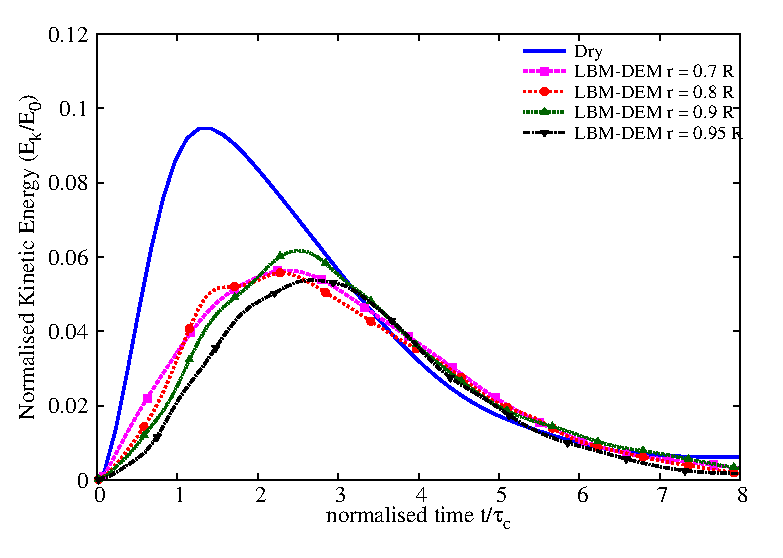
\includegraphics[width=\textwidth]{KE_a08_loose}
    \caption{Evolution of the total kinetic energy}
    \label{fig:KE_a08_loose}
\end{subfigure}
}\\
\makebox[\linewidth][c]{
\begin{subfigure}[t]{0.95\textwidth}
	\centering
    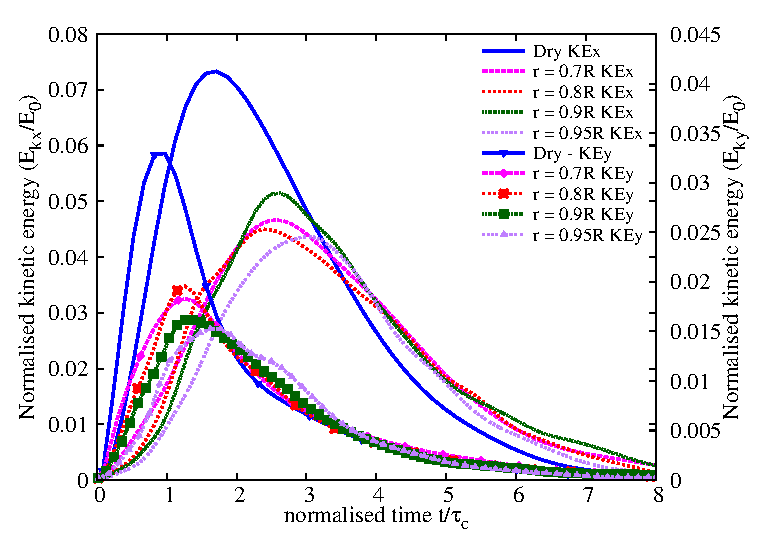
\includegraphics[width=\textwidth]{KExy_a08_loose}
    \caption{Evolution of horizontal and vertical kinetic energies}
    \label{fig:KExy_a08_loose}
\end{subfigure}
}
\caption{Effect of permeability on the evolution of kinetic energies with time 
for a granular column collapse in fluid (a = 0.8 \& loose packing)}
\label{fig:a08_loose_energy}
\end{figure}


\begin{figure}
	\centering
    \includegraphics[width=0.9\textwidth]{PE_a08_loose}
    \caption{Effect of permeability on the evolution of the potential energy 
    with time for a granular column collapse in fluid (a = 0.8 \& loose 
    packing)}
    \label{fig:PE_a08_loose}
\end{figure}


\begin{figure}
	\centering
    \includegraphics[width=0.9\textwidth]{Packing_Density_a08_loose}
    \caption{Effect of permeability on the evolution of packing density for a 
    granular column collapse in fluid (a = 0.8 \& loose initial packing)}
    \label{fig:Packing_Density_a08_loose}
\end{figure}

\begin{figure}
\centering
\makebox[\linewidth][c]{
\begin{subfigure}[t]{0.975\textwidth}
	\centering
    \includegraphics[width=\textwidth]{a08/PT_Dense_R095}
    \caption{Dense initial packing (79\%)}
    \label{fig:PT_Dense_R095}
\end{subfigure}
}\\
\makebox[\linewidth][c]{
\begin{subfigure}[t]{0.975\textwidth}
	\centering
    \includegraphics[width=\textwidth]{a08/PT_Loose_R095}
    \caption{Loose initial packing (83\%)}
    \label{fig:PT_Loose_R095}
\end{subfigure}
}
\caption{Effect of initial density on the deposit morphology
for a granular column collapse in fluid (a = 0.8). Dense vs loose initial 
packing fraction.}
\label{fig:Dense_Loose_PT}
\end{figure}


\begin{figure}
\centering
\makebox[\linewidth][c]{
\begin{subfigure}[t]{0.975\textwidth}
	\centering
    \includegraphics[width=\textwidth]{a08/Dense_a08_voro_tc}
    \caption{Dense initial packing (83\%)}
    \label{fig:Dense_a08_voro_tc}
\end{subfigure}
}\\
\makebox[\linewidth][c]{
\begin{subfigure}[t]{0.975\textwidth}
	\centering
    \includegraphics[width=\textwidth]{a08/Loose_a08_voro_tc}
    \caption{Loose initial packing (79\%)}
    \label{fig:Loose_a08_voro_tc}
\end{subfigure}
}
\caption{Evolution of packing fraction at $t = \tau_c$ for dense and loose 
initial packing fraction.}
\label{fig:Dense_Loose_voro}
\end{figure}




\section{Submarine granular flows down incline plane}

The flow of dense granular material is a common phenomenon in engineering 
predictions, such as avalanches, landslides, and debris-flow modelling. Despite 
the huge amount of research that has gone into describing the behaviour of 
granular flows, a constitutive equation that describes the overall behaviour of 
a flowing granular material is still lacking. The initiation and propagation of 
submarine granular flows depend mainly on the slope, density, and quantity of 
the material destabilised. Although certain macroscopic models are able to 
capture the simple mechanical behaviours, the complex physical mechanisms that 
occur at the grain scale, such as thydrodynamic instabilities, the formation of 
clusters, collapse, and transport, have largely been ignored~\citep{Topin2011}. 
The momentum transfer between the discrete and the continuous phases 
significantly affects the dynamics of the flow~\citep{Peker2007}. Grain-scale 
description of the granular material enriches the macro-scale variables,  which 
poorly account for the local rheology of the materials.  In order to describe 
the mechanism of saturated and/or immersed granular flows, it is important to 
consider both the dynamics of the solid phase and the role of the ambient 
fluid~\citep{Denlinger2001}. In particular, when the solid phase reaches a high 
volume fraction, it is important to consider the strong heterogeneity arising 
from the contact forces between the grains, the drag interactions which 
counteract the movement of the grains, and the hydrodynamic forces that reduce 
the weight of the solids inducing a transition from dense compacted to a dense 
suspended flow~\citep{Meruane2010}. The case of the collapse in presence of an 
interstitial fluid has been less studied. In this paper, we study the submarine 
granular flows in the inclined configuration. We study the effect of 
permeability, density and slope angle on the run-out evolution.



In this study, a 2D poly-disperse system ($d_{max}/d_{min} = 1.8$) of circular 
discs in fluid was used to understand the behaviour of granular flows on 
inclined planes (see~\Cref{fig:setup}). The soil column was modelled using 1000 
discs of density \SI{2650}{\kg\per\cubic\meter} and a contact friction angle of 
\SI{26}{\degree}. The collapse of the column was simulated inside a fluid with 
a density of \SI{1000}{\kg\per\cubic\meter}  and a kinematic viscosity of 
\SI{1e-6}{\square\meter\per\second}. The choice of a 2D geometry has the 
advantage of cheaper computational effort than a 3D case, making it feasible to 
simulate very large systems. A granular column of aspect ratio `a' of 0.8 was 
used. A hydrodynamic radius r = 0.9R was adopted during the LBM computations. 
Dry analyses were also performed to study the effect of hydrodynamic forces on 
the run-out distance.


\subsection{Effect of initial density}
The morphology of the granular deposits in fluid is shown to be mainly controlled by the initial volume fraction of the granular mass and not by the aspect ratio of the column~\citep{Rondon2011,Pailha2008}. In order to understand the influence of the initial packing density on the run-out behaviour, a dense sand column (initial packing density, $\Phi=83\%$) and a loose sand column ($\Phi=79\%$) were used. The granular columns collapse and flow down slopes of varying inclinations (\SI{2.5}{\degree}, \SI{5}{\degree} and \SI{7.5}{\degree}).

\begin{figure}
\centering
\includegraphics[width=0.97\columnwidth]{Runout_dense_slope}
\caption{Evolution of run-out with time (dense)}
\label{fig:run_dense}
\end{figure}

The evolution of run-out distances for a dense sand column with time in dry and submerged conditions for varying slope inclinations are presented in~\cref{fig:run_dense}. The run-out distance is longer in submerged condition than the dry condition for a flow on a horizontal surface. However, with increase in the slope angle the run-out in the fluid decreases.

Dense granular columns in fluid take a longer time to collapse and flow, due to the development of large negative pore-pressures, as the dense granular material dilates during the initial phase of the flow. The morphology of dense granular flows down slopes of varying inclinations at the critical time ($t=\tau_{c}=\sqrt{H/g}$, when the flow is fully mobilised) are shown in~\cref{fig:slope_dense}.

It can be seen that the viscous drag on the dense column tend to predominate over the influence of hydroplaning on the run-out behaviour. This influence can be observed in the smaller peak kinetic energy for granular column in fluid compared to it's dry counterpart (see~\Cref{fig:KE_dense}). With increase in slope angle, the volume of material that dilates increases. This results in large negative pore pressures and more viscous drag on the granular material. Hence, the difference in the run-out between the dry and the submerged condition, for a dense granular assembly, increases with increase in the slope angle.

\begin{figure}
\centering
\includegraphics[width=0.97\columnwidth]{KE_dense_slope}
\caption{Evolution of Kinetic Energy with time (dense case)}
\label{fig:KE_dense}
\end{figure}


\begin{figure}
\makebox[\linewidth][c]{
\begin{subfigure}[b]{0.95\textwidth}
	\centering
    \includegraphics[width=0.95\textwidth]{dense_slope/dense_slope25r09}
    \caption{Slope 2.5}
    \label{fig:ds2.5}
\end{subfigure}
}\\

\makebox[\linewidth][c]{
\begin{subfigure}[b]{0.95\textwidth}
	\centering
    \includegraphics[width=0.95\textwidth]{dense_slope/dense_slope5r09}
    \caption{Slope 5.0}
    \label{fig:ds5.0}
\end{subfigure}
}\\

\makebox[\linewidth][c]{
\begin{subfigure}[b]{0.95\textwidth}
	\centering
    \includegraphics[width=0.95\textwidth]{dense_slope/dense_slope75r09}
    \caption{Slope 7.5}
    \label{fig:ds7.5}
\end{subfigure}
}
\caption{Flow morphology at critical time for different slope angles (dense)}
\label{fig:slope_dense}
\end{figure}

In contrast to the dense granular columns, the loose granular columns (relative density $I_D=30 \%$) show longer run-out distance in immersed conditions (see~\Cref{fig:run_loose}). The run-out distance in fluid increases with increase in the slope angle compared to the dry cases. Loose granular material tends to entrain more water at the base of the flow front, creating a lubricating surface, which causes longer run-out distance (see~\Cref{fig:slope_loose}). The hydroplaning effect causes an increase in the velocity the loose condition in comparison with the dense condition (see~\Cref{fig:KE_loose}).

\begin{figure}
\centering
\includegraphics[width=0.97\columnwidth]{Runout_loose_slope}
\caption{Evolution of run-out with time (loose)}
\label{fig:run_loose}
\end{figure}

\begin{figure}
\makebox[\linewidth][c]{
\begin{subfigure}[b]{0.95\textwidth}
	\centering
    \includegraphics[width=0.95\textwidth]{loose_slope/loose_slope25r09}
    \caption{Slope 2.5}
    \label{fig:ls2.5}
\end{subfigure}
}\\

\makebox[\linewidth][c]{
\begin{subfigure}[b]{0.95\textwidth}
	\centering
    \includegraphics[width=0.95\textwidth]{loose_slope/loose_slope5r09}
    \caption{Slope 5.0}
    \label{fig:ls5.0}
\end{subfigure}
}\\

\makebox[\linewidth][c]{
\begin{subfigure}[b]{0.95\textwidth}
	\centering
    \includegraphics[width=0.95\textwidth]{loose_slope/loose_slope75r09}
    \caption{Slope 7.5}
    \label{fig:ls7.5}
\end{subfigure}
}
\caption{Flow morphology at critical time for different slope angles (loose)}
\label{fig:slope_loose}
\end{figure}


\begin{figure}
\centering
\includegraphics[width=0.97\columnwidth]{KE_loose_slope}
\caption{Evolution of Kinetic Energy with time (loose)}
\label{fig:KE_loose}
\end{figure}

The evolution of packing density (see~\Cref{fig:voro}) shows that dense and the 
loose conditions reach similar packing density. This indicates that the dense 
granular column dilates more and is susceptible to higher viscous drag forces. 
Where as in the loose condition, a positive pore-pressure is observed at the 
base of the flow, indicating entrainment of water at the base, i.e. 
hydroplaning resulting in longer run-out distance.

\begin{figure}
\centering
\includegraphics[width=0.97\columnwidth]{Voronoi_Slope_Dense_Loose}
\caption{Evolution of packing density with time}
\label{fig:voro}
\end{figure}


\subsection{Effect of permeability}

In DEM, the grain -- grain interaction is described based on the overlap 
between the grains at the contact surface. In a 3D granular assembly, the pore 
spaces between grains are interconnected. Whereas in a 2-D assembly, the grains 
are in contact with each other that result in a non-interconnected pore-fluid 
space. This causes a no flow condition in a 2-D case. In order to overcome this 
difficulty, a reduction in radius is assumed only during the LBM computation 
phase (fluid and fluid -- solid interaction). The reduction in radius allows 
interconnected pore space through which the surrounding fluid can flow. This 
technique has no effect on the grain -- grain interactions computed using DEM. 
See~\citet{Kumar2012} for more details about the relationship between reduction 
in radius and permeability of the granular assembly.


For a slope angle of \SI{5}{\degree}, the hydrodynamic radius of the loosely 
packed grains was varied from r = 0.7R (high permeability), 0.75R, 0.8R, 0.85R 
to 0.9R (low permeability). The run-out distance is found to increase with 
decrease in the permeability of the granular assembly (see~\Cref{fig:run5}). 
The run-out distance for high permeable conditions (r = 0.7R -- 0.8R) were 
lower than their dry counterparts. Although, decrease in permeability resulted 
in an increase in the run-out distance, no significant change in the run-out 
behaviour was observed for a hydrodynamic radius of up to 0.8R.

With further decrease in permeability (r = 0.85R and 0.9R), the run-out 
distance in the fluid was greater than the run-out observed in the dry 
condition. At very low permeability (r = 0.9R), granular material started to 
entrain more water at the base, which causes a reduction in the effective 
stress accompanied by a lubrication effect on the flowing granular media. This 
can be seen as a significant increase in the peak kinetic energy and the 
duration of the peak energy, in comparison with dry and high permeable 
conditions (see~\Cref{fig:KE5}).

The permeability of the granular column did not have an influence on the evolution of height during the flow. However, dry granular column tends to collapse more than the immersed granular column (see~\Cref{fig:height5}).

\begin{figure}
\centering
\includegraphics[width=0.97\columnwidth]{Runout_loose_5_slope}
\caption{Evolution of run-out with time for different permeability (loose slope \SI{5}{\degree})}
\label{fig:run5}
\end{figure}


\begin{figure}
\centering
\includegraphics[width=0.97\columnwidth]{Height_loose_5_slope}
\caption{Evolution of height with time for different permeability (loose slope \SI{5}{\degree})}
\label{fig:height5}
\end{figure}

\begin{figure}
\centering
\includegraphics[width=0.97\columnwidth]{KE_loose_5_slope}
\caption{Evolution of Kinetic Energy with time for different permeability (loose slope \SI{5}{\degree})}
\label{fig:KE5}
\end{figure}

Positive pore-pressure generation at the base of the flow was observed for low 
permeable conditions. Inspection of the local packing density showed 
entrainment of water at the base of the flow, which can also be observed by the 
steep decrease in the packing density (see~\Cref{fig:voro5}) for the very low 
permeability condition (r = 0.9R). At the end of the flow ($t \ge 3 \times 
\tau_c$), the excess pore-pressure dissipates and the granular material, 
irrespective of their permeability, reaches almost the same packing density.

\begin{figure}
\centering
\includegraphics[width=0.97\columnwidth]{Voronoi_5}
\caption{Evolution of packing density with time for different permeability (loose slope \SI{5}{\degree})}
\label{fig:voro5}
\end{figure}

\subsection{Tall columns}

\begin{figure}[htpb]
\centering
\includegraphics[width=0.9\textwidth]{LBM_DEM_a6}
\caption{Flow evolution of a granular column collapse in fluid (a = 6) on a 
horizontal surface}
\label{fig:LBM_DEM_a6}
\end{figure}


\begin{figure}
\makebox[\linewidth][c]{
\begin{subfigure}[b]{0.95\textwidth}
	\centering
    \includegraphics[width=0.95\textwidth]{a6/a6slope5t_0}
    \caption*{$t = 0\tau_c$}
    \label{fig:a6slope5t_0}
\end{subfigure}
}\\

\makebox[\linewidth][c]{
\begin{subfigure}[b]{0.95\textwidth}
	\centering
    \includegraphics[width=0.95\textwidth]{a6/a6slope5t_1tc}
    \caption*{$t = 1\tau_c$}
    \label{fig:a6slope5t_1tc}
\end{subfigure}
}\\
\makebox[\linewidth][c]{
\begin{subfigure}[b]{0.95\textwidth}
	\centering
    \includegraphics[width=0.95\textwidth]{a6/a6slope5t_3tc}
    \caption*{$t = 3\tau_c$}
    \label{fig:a6slope5t_3tc}
\end{subfigure}
}
\end{figure}
\begin{figure}
\ContinuedFloat
\makebox[\linewidth][c]{
\begin{subfigure}[b]{0.95\textwidth}
	\centering
    \includegraphics[width=0.95\textwidth]{a6/a6slope5t_6tc}
    \caption*{$t = 6\tau_c$}
    \label{fig:a6slope5t_6tc}
\end{subfigure}
}\\
\makebox[\linewidth][c]{
\begin{subfigure}[b]{0.95\textwidth}
	\centering
    \includegraphics[width=0.95\textwidth]{a6/a6slope5t_8tc}
    \caption*{$t = 8\tau_c$}
    \label{fig:a6slope5t_8tc}
\end{subfigure}
}
\caption{Flow evolution of a granular column collapse in fluid (a = 6) on a 
slope of 5\si{\degree}. Shows the velocity profile of fluid due to interaction 
with the grains (red - higher 
velocity).}
\label{fig:a6_slope_snapshots}
\end{figure}


\begin{figure}[htpb]
\centering
\includegraphics[width=0.9\textwidth]{Runout_a6_slope}
\caption{Evolution of run-out for a column collapse in fluid (a = 6) on a 
slope of 5\si{\degree}}
\label{fig:Runout_a6_slope}
\end{figure}

\begin{figure}[htpb]
\centering
\includegraphics[width=0.9\textwidth]{Height_a6_slope}
\caption{Evolution of height with time for a column collapse in fluid (a = 6) 
on a slope of 5\si{\degree}}
\label{fig:Height_a6_slope}
\end{figure}

\begin{figure}
\centering
\makebox[\linewidth][c]{
\begin{subfigure}[t]{0.8\textwidth}
	\centering
    \includegraphics[width=\textwidth]{KE_a6_slope}
    \caption{Evolution of the total kinetic energy}
    \label{fig:KE_a6_slope}
\end{subfigure}
}\\
\makebox[\linewidth][c]{
\begin{subfigure}[t]{0.95\textwidth}
	\centering
    \includegraphics[width=\textwidth]{PE_a6_slope}
    \caption{Evolution of the total potential energy}
    \label{fig:PE_a6_slope}
\end{subfigure}
}
\caption{Evolution of the kinetic and the potential energy with time for a 
granular 
column collapse in fluid (a = 6) on a slope of 5\si{\degree}}
\label{fig:a6_KEPE}
\end{figure}


\begin{figure}
\centering
\makebox[\linewidth][c]{
\begin{subfigure}[t]{0.8\textwidth}
	\centering
    \includegraphics[width=\textwidth]{KEx_a6_slope}
    \caption{Evolution of the vertical kinetic energy}
    \label{fig:KEx_a6_slope}
\end{subfigure}
}\\
\makebox[\linewidth][c]{
\begin{subfigure}[t]{0.95\textwidth}
	\centering
    \includegraphics[width=\textwidth]{KEy_a6_slope}
    \caption{Evolution of the horizontal kinetic energy}
    \label{fig:KEy_a6_slope}
\end{subfigure}
}
\caption{Evolution of the kinetic energies with time for a granular 
column collapse in fluid (a = 6) on a slope of 5\si{\degree}}
\label{fig:a6_KEPE}
\end{figure}


\begin{figure}
\makebox[\linewidth][c]{
\begin{subfigure}[b]{0.95\textwidth}
	\centering
    \includegraphics[width=0.95\textwidth]{a6/a6_slope5_6tc}
    \caption*{$t = 6\tau_c$}
    \label{fig:a6_slope5_6tc}
\end{subfigure}
}\\
\makebox[\linewidth][c]{
\begin{subfigure}[b]{0.95\textwidth}
	\centering
    \includegraphics[width=0.95\textwidth]{a6/a6_slope5_8tc}
    \caption*{$t = 8\tau_c$}
    \label{fig:a6_slope5_8tc}
\end{subfigure}
}
\caption{Packing density of a granular column collapse in fluid (a = 6) on a 
slope of 5\si{\degree}.}
\label{fig:a6_slope_voro}
\end{figure}

\subsection{Summary}

Two-dimensional LB-DEM simulations were performed to understand the behaviour 
of submarine granular flows. Unlike dry granular collapse, the run-out 
behaviour in fluid is dictated by the initial volume fraction. Granular columns 
with loose packing tend to flow longer in comparison to dense columns, due to 
entrainment of water at the base resulting in lubrication. The loose column 
when it starts flowing expands and ejects liquid, leading to a partial 
fluidization of the material. However, with increase in the slope angle, the 
run-out in fluid is influenced by the viscous drag on the granular materials. 
The run-out distance in fluid increases with decrease in permeability. More 
research work is required to characterise the flow behaviour of granular 
materials, especially in submerged conditions.
